
\section{Sequencer operation}



In normal operation, the sequencer will loop through all the steps in a cyclic fashion, the current step can be seen by the indicated LED. In order to to create a rythm, the user can activate the desired steps by activating the correspondant switch. The activated steps are indicated by their correspondant LEDs being on.  

The sound output of the signal is a DC biased square wave outputted by an IO pin of the Basys 2 Board, this should be connected to and external powered speaker in order to the sound to be apmplified and filtered.


Figure~\ref{fig:bdbasys2} shows the Basys 2 peripherals that the user can use in order to interact with the sequencer.

\begin{figure}[!h]
  \centerline{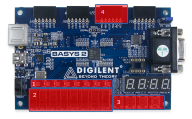
\includegraphics[scale=1]{bdboard.png}}
  \vspace{0cm}\caption{Basys 2 board peripherals}
  \label{fig:bdbasys2}
\end{figure}

\section{Implementation}


Since the sequencer depends on multiple time-dependant routines and there is no trivial way to deal with this on the picoversat controller (because of the lack of interrupts), the main logic is divided into two routines: one for the main sequencer loop, implemented as a standalone peripheral, the ''Sequencer loop controller'', and other for the reading and debouncing of the pushbuttons and for keeping track of the frequency and loop values.


\noindent All the peripherals and modules are interconnected as described in the following picture:

\begin{figure}[!htbp]
  \centerline{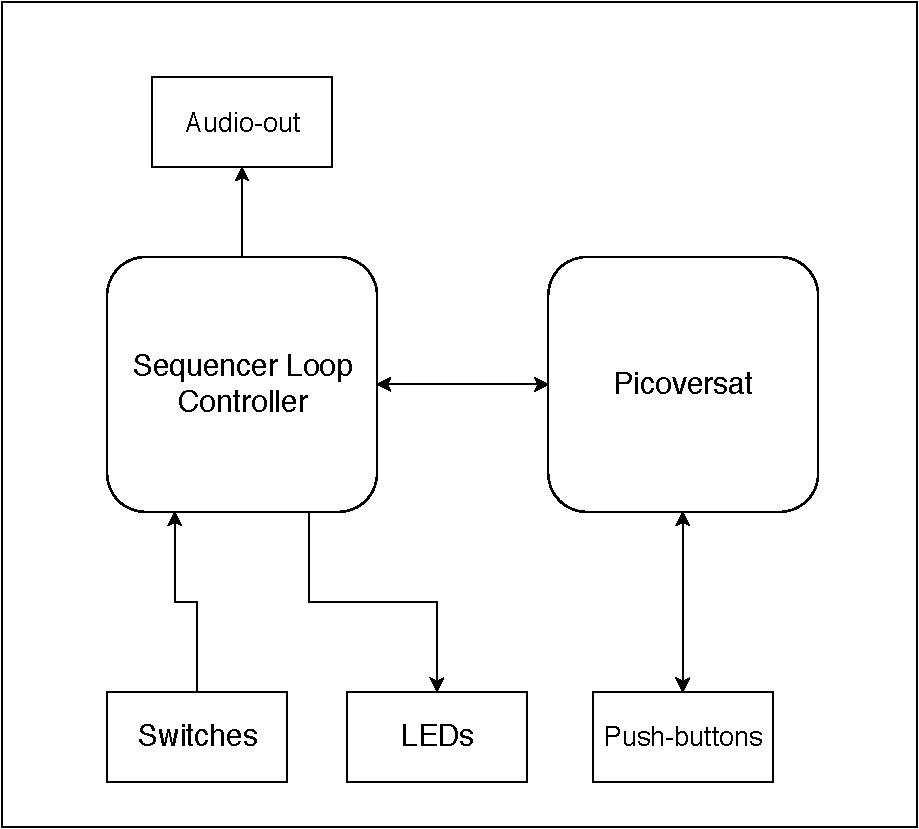
\includegraphics[scale=0.5]{periphmoddiag.pdf}}
  \vspace{0cm}\caption{Basys 2 board peripherals}
  \label{fig:periphmoddiag}
\end{figure}


\subsection{Sequencer Loop Controller}


\noindent The sequencer loop controller is used to generate the sequencer loop. The loop and note frequency can be set by using the \textit{freq} input and by selecting the according selector signal.
The Sequencer loop controller will output a square wave corresponding to the loop ouput. The led outputs are directly connected to the LED driver peripheral and send information about the current and selected note. 

\noindent The sequencer loop controller operation is described by the fluxogram on Picture \ref{fig:fluxloop}.


\begin{figure}[!htbp]
    \centerline{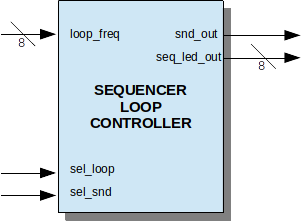
\includegraphics[scale=0.5]{SequencerLoopcontroler.png}}
    \vspace{0cm}\caption{PicoVersat SoC with two peripherals}
    \label{fig:periphs}
\end{figure}

% Please add the following required packages to your document preamble:
% \usepackage{booktabs}
\begin{table}[!htbp]
    \centering
    \caption{Sequencer Loop Controller Inputs}
    \label{tab:slcIn}
    \begin{tabular}{@{}lcl@{}}
    \toprule
    Name      & \multicolumn{1}{l}{\#bits} & Description                                    \\ \midrule
    freq & 8                          & Loop Period / Note Frequency                                    \\
    sel\_loop & 1                          & Loop period select signal (address decoder)    \\
    sel\_snd  & 1                          & Note frequency select signal (address decoder) \\ \bottomrule
    \end{tabular}
    \end{table}

    % Please add the following required packages to your document preamble:
% \usepackage{booktabs}
\begin{table}[!htbp]
    \centering
    \caption{Sequencer Loop Controller Outputs}
    \label{tab:slcOut}
    \begin{tabular}{@{}lcl@{}}
    \toprule
    Name          & \multicolumn{1}{l}{\#bits} & Description             \\ \midrule
    snd\_out      & 1                          & Audio Output            \\
    seq\_led\_out & 8                          & Current note led output \\ \bottomrule
    \end{tabular}
    \end{table}

    \begin{figure}[!htbp]
      \centerline{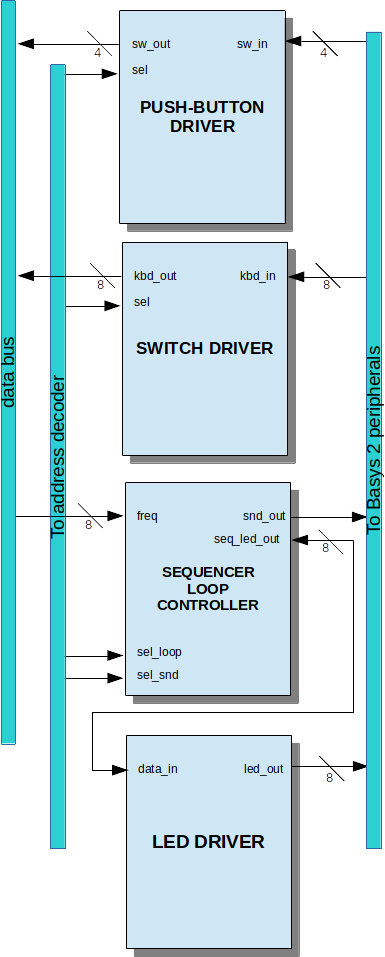
\includegraphics[scale=0.5]{periphs_interconn.png}}
      \vspace{0cm}\caption{PicoVersat SoC with two peripherals}
      \label{fig:periphs}
  \end{figure}

\begin{figure}[!htbp]
  \centerline{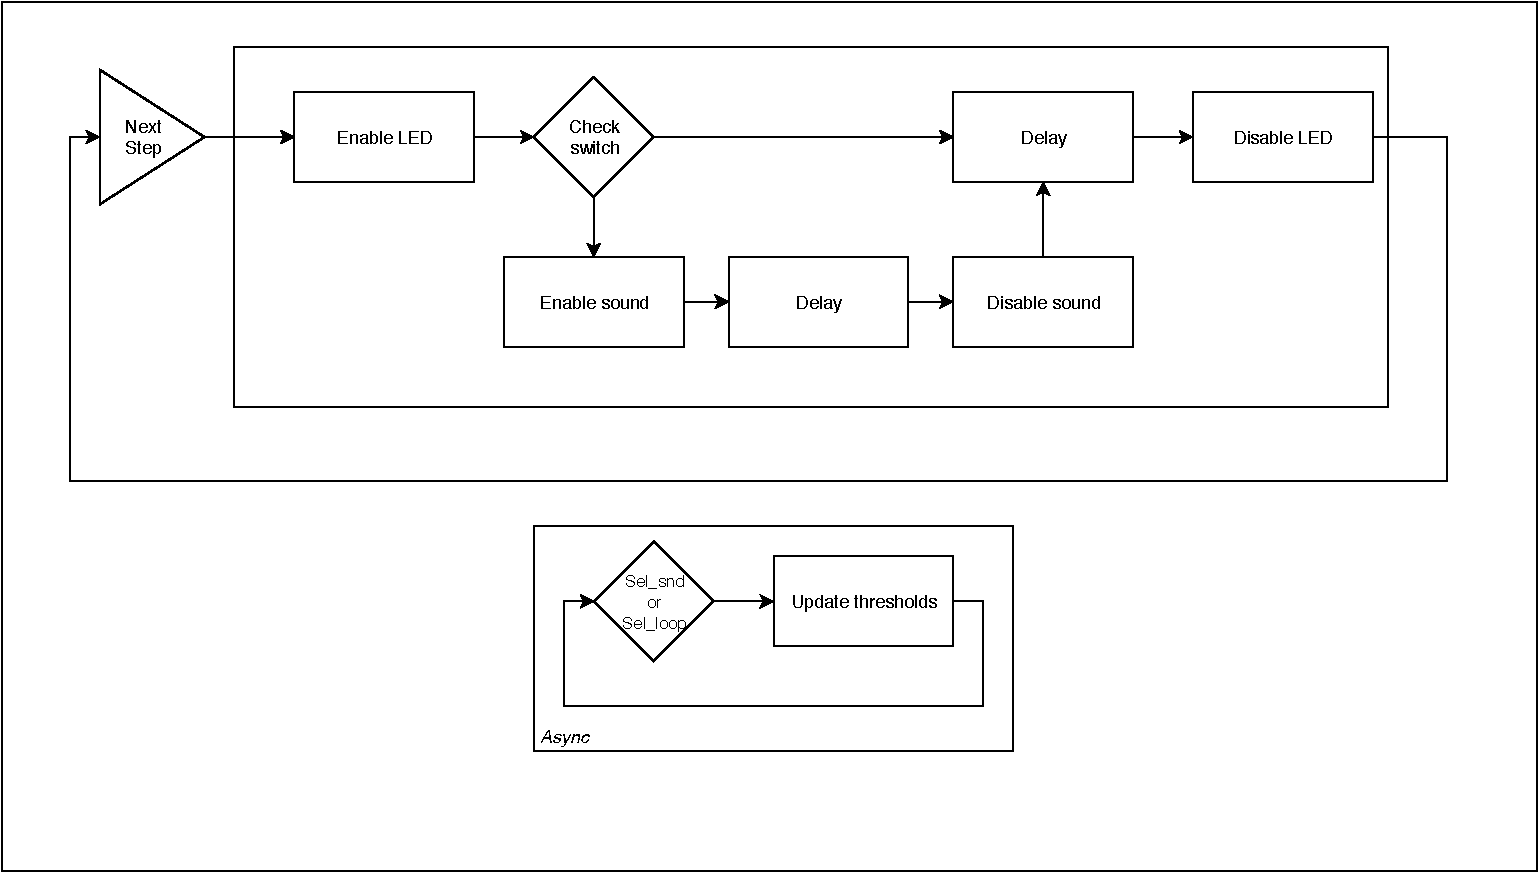
\includegraphics[scale=0.4]{Sequencer_loop_controller_flux.pdf}}
  \vspace{0cm}\caption{Sequencer Loop controler fluxogram.}
  \label{fig:bd}
\end{figure}


\subsection{Picoversat}

For reading the pushbuttons, debouncing and managing loop and sound frequencies, the picoversat SoC was used. The Sequencer Loop Controler is connected to the picoversat data bus and the loop and sound frequency registers are mapped in memory. For this, the picoversat address decoder was altered so that the sequencer loop controller's registers can be accessed. This was also done for the push-buttons.

Some auxiliary modules were also added to the picoversat:

\subsubsection{General Purpose Register File}

This peripheral contains a 16x32bit register file that can be used by user
programs. Refer to the picoversat manual for more information about this peripheral. 


\subsubsection{Debug Printer}

This peripheral can be used by user programs to print characters, mainly for
debug purposes. Refer to the picoversat manual for more information about this peripheral.


All of the aforementioned peripherals connect to the picoversat as described below:

\begin{figure}[!htbp]
  \centerline{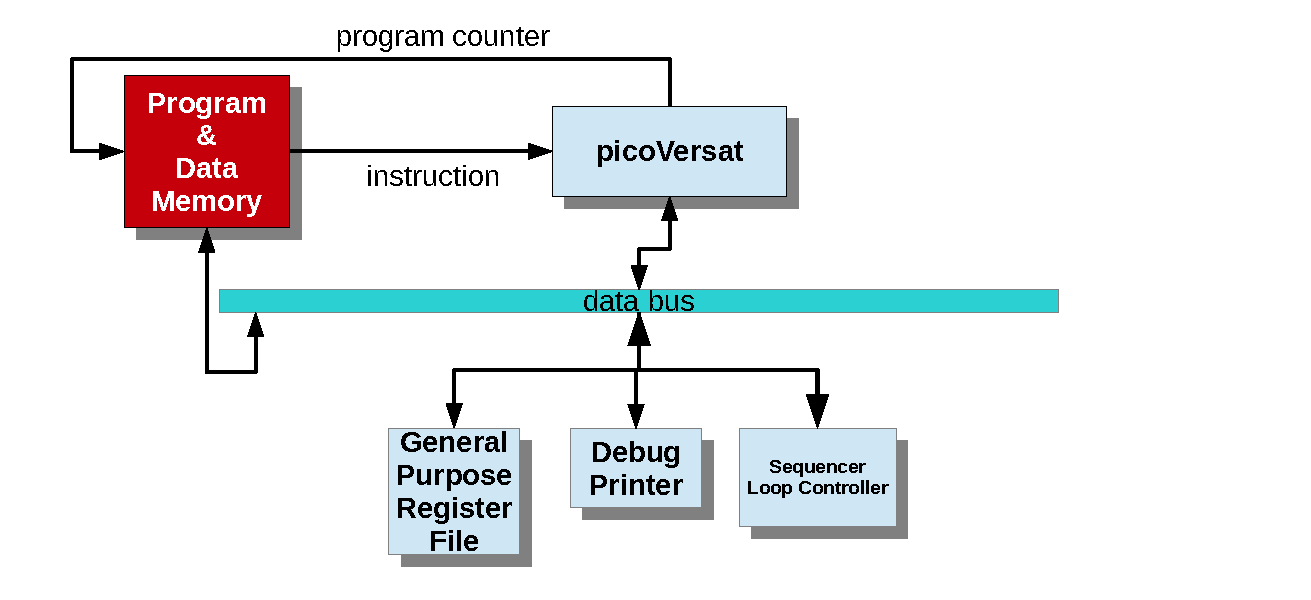
\includegraphics[scale=0.7]{periphs.pdf}}
  \vspace{0cm}\caption{PicoVersat SoC with two peripherals}
  \label{fig:periphs}
\end{figure}

The final memory map is represented on following table:

% Please add the following required packages to your document preamble:
% \usepackage{booktabs}
\begin{table}[!htbp]
  \centering
  \caption{Memmory map}
  \label{tab:memmap}
  \begin{tabular}{@{}lcccl@{}}
  \toprule
  Mnemonic   & \multicolumn{1}{l}{Address} & \multicolumn{1}{l}{Read/Write} & \multicolumn{1}{l}{Read/Write Latency} & Description                                           \\ \midrule
  SND\_BASE  & 0x25E                       & Write only                     & 0                                      & Sound frequency address for sequencer loop controller \\
  LOOP\_BASE & 0x25C                       & Write only                     & 0                                      & Loop frequency address for sequencer loop controller  \\
  PUSH\_BASE & 0x25A                       & Read only                      & 0                                      & Push-button peripheral                                \\
  CPRT\_BASE & 0x258                       & Read only                      & N/A                                    & Debug printer peripheral                              \\
  REGF\_BASE & 0x200                       & Read+Write                     & 0                                      & Register file peripheral                              \\
  PROG\_BASE & 0x0                         & Read+Write                     & 1                                      & User program and data                                 \\ \bottomrule
  \end{tabular}
  \end{table}

\subsubsection{Software}

The picoversat was firstly developed in C and cross-compiled into picoversat assembly using the lcc compiler. Unfortunately due to some setbacks with the lcc code file size and picoversat's memory size, the code was implemented again from scratch in assembly. This resulted in a smaller and better optimized program.
The general program logic is represented below:

\begin{figure}[htbp]
  \centerline{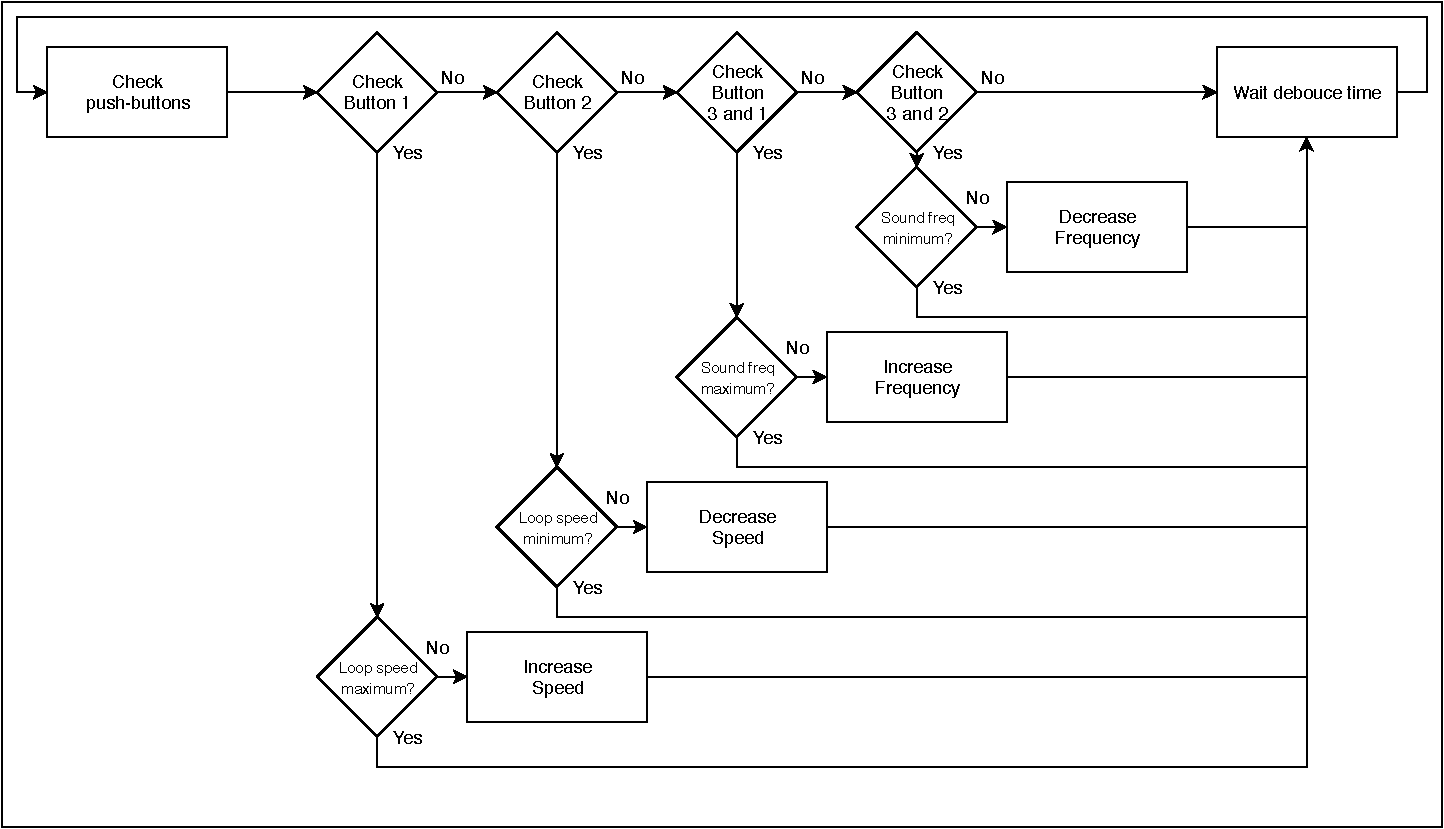
\includegraphics[scale=0.4]{picoversat_flux.pdf}}
  \vspace{0cm}\caption{Picoversat code fluxogram.}
  \label{fig:fluxloop}
\end{figure}

